\bookchapter{الفصل 49: تجهيز بيئة التطوير — Android Studio وأول مشروع}

\chapterintro{من أراد أن يُتقن العمل أتقن أدواته أولًا. في هذا الفصل سنجعل «المطبخ» جاهزًا: نثبّت Android Studio، ونشغّل المحاكي بنجاح، وننشئ أول مشروع Android في حياتك، ثم نفكك بنية المشروع لنفهمها فهمًا واضحًا. وبعد تجهيز البيئة ستشاهد لأول مرة كودك يتحول إلى زر يمكنك النقر عليه — لحظة يتذكرها كثيرون طوال العمر.}

\booksection{أولًا: تثبيت Android Studio}

Android Studio هي بيئة التطوير المتكاملة (IDE) الرسمية من جوجل، مجانية وشاملة الوظائف: كتابة الكود، ومعاينة الواجهة، وتصحيح الأخطاء، وحزم التطبيق، كل ذلك في مكان واحد. التثبيت في أربع خطوات:

\begin{enumerate}
  \item افتح الموقع الرسمي developer.android.com/studio ونزّل أحدث إصدار مستقر (في أغسطس 2026 كان الإصدار الذي يلي Narwhal، وهو متاح لأنظمة Windows/Mac/Linux)؛
  \item شغّل ملف التثبيت واختر «التالي» طوال الطريق — سيثبّت المعالج تلقائيًا مكونات Android SDK والمحاكي؛
  \item عند أول تشغيل نزّل مكونات SDK حسب التعليمات (اترك الخيارات الافتراضية كما هي؛ قد يستغرق الأمر بضع دقائق وبضعة جيجابايت من المساحة)؛
  \item بعد الانتهاء ستظهر لك صفحة الترحيب — تهانينا، أصبح «المطبخ» جاهزًا.
\end{enumerate}

\begin{tcbwarn}{تنبيه: خذ متطلبات العتاد بعين الاعتبار}
Android Studio «آكلة للذاكرة»: يُنصح بذاكرة 16 جيجابايت في الحد الأدنى (يعمل بـ 8 جيجابايت لكن المحاكي سيتقطع كثيرًا)، مع حجز أكثر من 20 جيجابايت على القرص، ومعالج يدعم المحاكاة الافتراضية (فعّل VT-x/AMD-V من BIOS). إذا كان حاسوبك قديمًا فعلًا، يمكنك استخدام «التصحيح على جهاز حقيقي» بدلًا من المحاكي (سأشرحه في القسم الرابع من هذا الفصل)، وقد تكون التجربة عندها أكثر سلاسة.

\end{tcbwarn}

\booksection{ثانيًا: إنشاء أول مشروع لك}

من صفحة الترحيب انقر New Project واختر قالب Empty Activity (أنظف قالب للمبتدئين)، ثم املأ ثلاثة أشياء:

\begin{center}
\begin{tabularx}{\linewidth}{|X|X|X|}
\hline
\textbf{بند الإعداد} & \textbf{ماذا تملأ} & \textbf{الشرح} \tabularnewline
\hline
Name & My First App & اسم التطبيق، ويظهر على الشاشة الرئيسية للهاتف \tabularnewline
Package name & com.example.myfirstapp & معرّف فريد عالميًا، والعادة هي «عكس ترتيب اسم النطاق»، اتركه الافتراضي في البداية \tabularnewline
Minimum SDK & API 26(Android 8.0) & الحد الأدنى للإصدارات المدعومة، ويغطي أكثر من 95\% من الأجهزة \tabularnewline
\hline
\end{tabularx}
\end{center}

\begin{center}\small\color{gray}الأشياء الثلاثة المطلوب ملؤها عند إنشاء المشروع\end{center}

بعد النقر على Finish سيستخدم Android Studio أداة Gradle لتنزيل الاعتماديات وبناء المشروع تلقائيًا (المرة الأولى تستغرق بضع دقائق، وبعدها تصبح أسرع بكثير). وبعد اكتمال البناء سيكون لديك تطبيق قابل للتشغيل — وإن كان لا يعرض سوى سطر “Hello Android!”.

\begin{tcbinfo}{نصيحة: أسرار اسم الحزمة}
اسم الحزمة (package name) يشبه «رقم الهوية» للتطبيق؛ لا يجوز تكراره عالميًا، وبعد النشر لا يمكن تغييره. للتمارين الشخصية يكفي com.example.xxx؛ أما المنتجات الرسمية فيجب أن تحمل عكس ترتيب نطاقك الخاص (مثل com.اسمك.اسمالتطبيق). لا تنشر تطبيقًا باسم com.example — فالمتجر سيرفضه.

\end{tcbinfo}

\booksection{ثالثًا: لنشغّله: المحاكي والجهاز الحقيقي}

بعد كتابة الكود، نحتاج «هاتفًا» نشغّل عليه. أمامك خياران:

\booksubsection{المحاكي (Emulator)}

المحاكي ينشئ هاتف Android افتراضيًا داخل حاسوبك. في Android Studio افتح Device Manager ثم Create Device، واختر جهازًا (يُنصح بسلسلة Pixel) ثم صورة نظام (من النوع الذي يتضمن Google APIs) ثم نزّلها وشغّلها. بعدها انقر المثلث الأخضر Run في شريط الأدوات، وخلال ثوانٍ ستظهر على شاشة «الهاتف» واجهة تطبيقك.

\booksubsection{التصحيح على جهاز حقيقي (الأكثر توصية)}

الجهاز الحقيقي يبقى بيئة الاختبار الأكثر واقعية — انسياب اللمس والشبكة الحقيقية والمستشعرات الحقيقية لا يشبهها المحاكي فيها شيء. والتصحيح على هاتف Android حقيقي بسيط جدًا:

\begin{enumerate}
  \item في الهاتف افتح [الإعدادات] > [حول الهاتف]، وانقر «رقم الإصدار» 7 مرات متتالية لتفعيل «خيارات المطوّر»؛
  \item في [خيارات المطوّر] فعّل تصحيح USB؛
  \item وصّل الهاتف بالحاسوب بكابل بيانات، واختر «السماح بتصحيح USB» من النافذة المنبثقة؛
  \item عُد إلى Android Studio وسيظهر هاتفك في قائمة الأجهزة المنسدلة في شريط الأدوات، ثم انقر Run.
\end{enumerate}

\textbf{تحذير من الفخاخ: لا تُبقِ تصحيح USB مفعّلًا دائمًا}\par

تصحيح USB يشبه فتح «باب خلفي» لحاسوبك. عند الشحن في الأماكن العامة أو الاتصال بحواسيب لا تثق بها، احرص على إيقاف تصحيح USB لمنع الآخرين من قراءة بياناتك عبره. أغلقه بعد كل استخدام أثناء التطوير، حتى يصبح عادة راسخة.

\booksection{رابعًا: تفكيك بنية المشروع: ما وظيفة كل ملف}

عند فتح المشروع لأول مرة قد تُذهلك شجرة الملفات على اليسار. لا تقلق؛ في التطوير اليومي ستقضي 90\% من وقتك مع الملفات التالية فقط:

\begin{center}
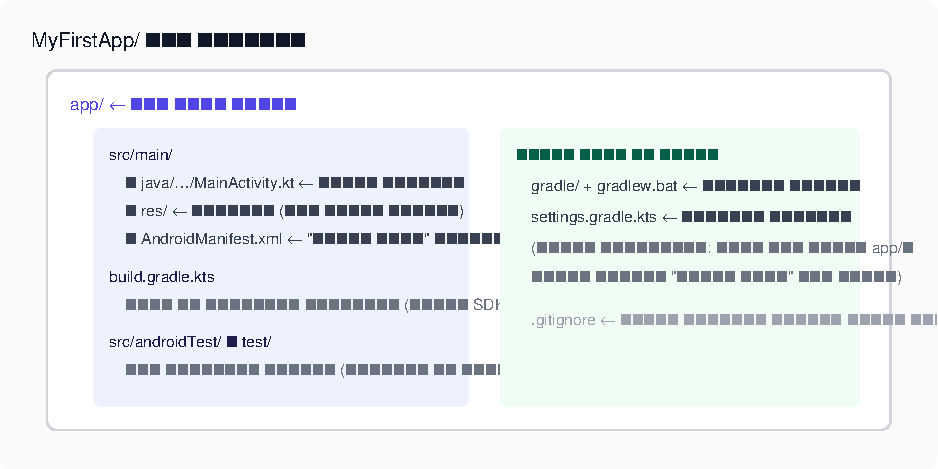
\includegraphics[width=0.92\linewidth]{figures/fig-di-si-shi-jiu-zhang-1}
\\[2pt]\small الشكل 2: بنية المشروع التي يجب على المبتدئ فهمها (القاعدة الذهبية: لا تلمس سوى مجلد app/)
\end{center}

\begin{itemize}
  \item MainActivity.kt: «البوابة الرئيسية» للتطبيق. عندما ينقر المستخدم على الأيقونة فهو أول ما يُيقظ. في القوالب الحالية مسؤوليته عرض "Hello Android!".
  \item AndroidManifest.xml: «سجل القيد» للتطبيق — يصرّح باسم التطبيق وأيقونته وصفحاته والأذونات التي يحتاجها (الكاميرا، تحديد الموقع وغيرها).
  \item مجلد res/: مستودع الموارد، يخزن الصور والأيقونات والنصوص والألوان. وضع النصوص في ملفات الموارد بدلًا من تثبيتها في الكود عادة جيدة في تطوير Android (يسهل بها تغيير اللغة والمظهر).
  \item build.gradle.kts: وصفة البناء — تصريح الحد الأدنى للإصدارات والاعتماديات المطلوبة (مثل Compose).
\end{itemize}

\booksection{خامسًا: تجربة أولى: استبدل “Hello” باسمك}

افتح MainActivity.kt وسترى الكود الذي ولّده قالب Compose. ابحث عن السطر Text(“Hello Android!”) واستبدل ما بين علامتي التنصيص باسمك، مثل Text(“مرحبًا، أنا أحمد! هذا أول تطبيق لي”)، ثم اضغط Ctrl+R (أو Cmd+R على Mac) لإعادة التشغيل. وبعد ثوانٍ سيظهر اسمك على المحاكي.

\begin{lstlisting}[language=Kotlin]
setContent {
    MyFirstAppTheme {
        Surface(modifier = Modifier.fillMaxSize()) {
            // v غيّر هنا إلى النص الذي تريده
            Text("مرحبًا أحمد! هذا أول تطبيق لي")
        }
    }
}
\end{lstlisting}

تهانينا؛ لقد أكملت دورة كاملة “تعديل الكود تجميع تثبيت تشغيل”. هذه الدورة هي روتين التطوير اليومي مستقبلًا. اجعل الحديد ساخنًا وجرّب تعديل أشياء أخرى: كبّر حجم الخط أو غيّر اللون — في الفصل القادم سنتعلم من أين تأتي هذه “التعاويذ”.

\booksection{سادسًا: إسعافات أولية للأخطاء الشائعة: “قسم الطوارئ” لأول أسبوعين للمبتدئ}

في مرحلة تجهيز البيئة وأول بناء ستقابل على الأرجح الأخطاء الثلاثة التالية. لا تذعر؛ لكل منها علاج:

\begin{center}
\begin{tabularx}{\linewidth}{|X|X|X|}
\hline
\textbf{شكل الخطأ} & \textbf{السبب الشائع} & \textbf{العلاج} \tabularnewline
\hline
فشل مزامنة Gradle / بطء تنزيل الاعتماديات & ضعف الوصول الشبكي إلى المستودعات & اضبط Gradle لاستخدام مستودعات مرايا محلية (مرايا maven من Aliyun/Tencent Cloud)، وابحث في الإنترنت عن «مرايا Gradle الصينية» واتبع الشرح \tabularnewline
مكونات SDK ناقصة & تجاوز تنزيل SDK أثناء التثبيت & افتح Settings ثم SDK Manager وثبّت المنصات والأدوات الناقصة \tabularnewline
فشل تشغيل المحاكي / شاشة سوداء & المحاكاة الافتراضية غير مفعّلة أو الصورة تالفة & فعّل VT-x/AMD-V من BIOS؛ واحذف المحاكي وأنشئه من جديد؛ أو استخدم التصحيح على جهاز حقيقي مباشرة \tabularnewline
\hline
\end{tabularx}
\end{center}

\begin{center}\small\color{gray}جدول الإسعافات الأولية لأخطاء بيئة المبتدئين\end{center}

\begin{tcbinfo}{نصيحة: منهجية البحث عن الأخطاء}
السطر الأول من رسالة الخطأ هو الأثمن — انسخه كما هو في محرك البحث وأضف الكلمة المفتاحية “android studio”. لا تبحث عن أسئلة عامة مثل “لا أستطيع تجهيز البيئة ماذا أفعل”، بل عن أخطاء محددة مثل “Gradle sync failed: Could not resolve com.android.tools.build”. السؤال الدقيق وحده يعطي الجواب الدقيق.

\end{tcbinfo}

\begin{tcbpractice}{لنتجرب: أكمل قائمة "طقوس التطوير" الخاصة بك}
(1) ثبّت Android Studio وشغّل المحاكي بنجاح؛ (2) شغّل تطبيقك على جهاز حقيقي مرة واحدة واحتفظ بلقطة شاشة؛ (3) غيّر نص Hello إلى اسمك؛ (4) اضغط المشروع في ملف مضغوط واحفظ نسخة احتياطية. بعد هذه الخطوات الأربع يمكنك إعلان أصدقائك: صرت مطوّر Android أيضًا (ولقطة الشاشة هي الدليل).

\end{tcbpractice}

\begin{tcbsummary}{خلاصة الفصل}
\begin{itemize}
  \item Android Studio = بيئة التطوير الرسمية المجانية؛ يُنصح بذاكرة 16 جيجابايت + 20 جيجابايت قرص + تفعيل المحاكاة الافتراضية
  \item عناصر المشروع الجديد الثلاثة: الاسم، واسم الحزمة (فريد عالميًا ولا تنشر بـ com.example)، والحد الأدنى للـ SDK (ابتداءً من API 26)
  \item طريقتان للتشغيل: المحاكي (هاتف افتراضي داخل الحاسوب) والجهاز الحقيقي (فعّل تصحيح USB وتذكّر إيقافه بعد الانتهاء)
  \item قاعدة المشروع: لا تلمس سوى مجلد app/ — MainActivity.kt هو البوابة، وManifest سجل القيد، وres/ مستودع الموارد
  \item روتين التطوير = تعديل الكود Run مشاهدة النتيجة، بالتكرار المستمر
\end{itemize}

\end{tcbsummary}
